\documentclass[twoside]{book}

% Packages required by doxygen
\usepackage{fixltx2e}
\usepackage{calc}
\usepackage{doxygen}
\usepackage[export]{adjustbox} % also loads graphicx
\usepackage{graphicx}
\usepackage[utf8]{inputenc}
\usepackage{makeidx}
\usepackage{multicol}
\usepackage{multirow}
\PassOptionsToPackage{warn}{textcomp}
\usepackage{textcomp}
\usepackage[nointegrals]{wasysym}
\usepackage[table]{xcolor}

% Font selection
\usepackage[T1]{fontenc}
\usepackage[scaled=.90]{helvet}
\usepackage{courier}
\usepackage{amssymb}
\usepackage{sectsty}
\renewcommand{\familydefault}{\sfdefault}
\allsectionsfont{%
  \fontseries{bc}\selectfont%
  \color{darkgray}%
}
\renewcommand{\DoxyLabelFont}{%
  \fontseries{bc}\selectfont%
  \color{darkgray}%
}
\newcommand{\+}{\discretionary{\mbox{\scriptsize$\hookleftarrow$}}{}{}}

% Page & text layout
\usepackage{geometry}
\geometry{%
  a4paper,%
  top=2.5cm,%
  bottom=2.5cm,%
  left=2.5cm,%
  right=2.5cm%
}
\tolerance=750
\hfuzz=15pt
\hbadness=750
\setlength{\emergencystretch}{15pt}
\setlength{\parindent}{0cm}
\setlength{\parskip}{3ex plus 2ex minus 2ex}
\makeatletter
\renewcommand{\paragraph}{%
  \@startsection{paragraph}{4}{0ex}{-1.0ex}{1.0ex}{%
    \normalfont\normalsize\bfseries\SS@parafont%
  }%
}
\renewcommand{\subparagraph}{%
  \@startsection{subparagraph}{5}{0ex}{-1.0ex}{1.0ex}{%
    \normalfont\normalsize\bfseries\SS@subparafont%
  }%
}
\makeatother

% Headers & footers
\usepackage{fancyhdr}
\pagestyle{fancyplain}
\fancyhead[LE]{\fancyplain{}{\bfseries\thepage}}
\fancyhead[CE]{\fancyplain{}{}}
\fancyhead[RE]{\fancyplain{}{\bfseries\leftmark}}
\fancyhead[LO]{\fancyplain{}{\bfseries\rightmark}}
\fancyhead[CO]{\fancyplain{}{}}
\fancyhead[RO]{\fancyplain{}{\bfseries\thepage}}
\fancyfoot[LE]{\fancyplain{}{}}
\fancyfoot[CE]{\fancyplain{}{}}
\fancyfoot[RE]{\fancyplain{}{\bfseries\scriptsize Generated by Doxygen }}
\fancyfoot[LO]{\fancyplain{}{\bfseries\scriptsize Generated by Doxygen }}
\fancyfoot[CO]{\fancyplain{}{}}
\fancyfoot[RO]{\fancyplain{}{}}
\renewcommand{\footrulewidth}{0.4pt}
\renewcommand{\chaptermark}[1]{%
  \markboth{#1}{}%
}
\renewcommand{\sectionmark}[1]{%
  \markright{\thesection\ #1}%
}

% Indices & bibliography
\usepackage{natbib}
\usepackage[titles]{tocloft}
\setcounter{tocdepth}{3}
\setcounter{secnumdepth}{5}
\makeindex

% Hyperlinks (required, but should be loaded last)
\usepackage{ifpdf}
\ifpdf
  \usepackage[pdftex,pagebackref=true]{hyperref}
\else
  \usepackage[ps2pdf,pagebackref=true]{hyperref}
\fi
\hypersetup{%
  colorlinks=true,%
  linkcolor=blue,%
  citecolor=blue,%
  unicode%
}

% Custom commands
\newcommand{\clearemptydoublepage}{%
  \newpage{\pagestyle{empty}\cleardoublepage}%
}

\usepackage{caption}
\captionsetup{labelsep=space,justification=centering,font={bf},singlelinecheck=off,skip=4pt,position=top}

%===== C O N T E N T S =====

\begin{document}

% Titlepage & ToC
\hypersetup{pageanchor=false,
             bookmarksnumbered=true,
             pdfencoding=unicode
            }
\pagenumbering{roman}
\begin{titlepage}
\vspace*{7cm}
\begin{center}%
{\Large My Project }\\
\vspace*{1cm}
{\large Generated by Doxygen 1.8.11}\\
\end{center}
\end{titlepage}
\clearemptydoublepage
\tableofcontents
\clearemptydoublepage
\pagenumbering{arabic}
\hypersetup{pageanchor=true}

%--- Begin generated contents ---
\chapter{Hierarchical Index}
\section{Class Hierarchy}
This inheritance list is sorted roughly, but not completely, alphabetically\+:\begin{DoxyCompactList}
\item \contentsline{section}{Fruit}{\pageref{classFruit}}{}
\begin{DoxyCompactList}
\item \contentsline{section}{Apple}{\pageref{classApple}}{}
\item \contentsline{section}{Grape}{\pageref{classGrape}}{}
\item \contentsline{section}{Orange}{\pageref{classOrange}}{}
\end{DoxyCompactList}
\item \contentsline{section}{List}{\pageref{classList}}{}
\item \contentsline{section}{List\+:\+:Node}{\pageref{structList_1_1Node}}{}
\end{DoxyCompactList}

\chapter{Class Index}
\section{Class List}
Here are the classes, structs, unions and interfaces with brief descriptions\+:\begin{DoxyCompactList}
\item\contentsline{section}{\hyperlink{structnode}{node} }{\pageref{structnode}}{}
\item\contentsline{section}{\hyperlink{structnode1}{node1} }{\pageref{structnode1}}{}
\item\contentsline{section}{\hyperlink{structnode__info}{node\+\_\+info} }{\pageref{structnode__info}}{}
\end{DoxyCompactList}

\chapter{File Index}
\section{File List}
Here is a list of all files with brief descriptions\+:\begin{DoxyCompactList}
\item\contentsline{section}{\hyperlink{Lab1_8c}{Lab1.\+c} }{\pageref{Lab1_8c}}{}
\end{DoxyCompactList}

\chapter{Class Documentation}
\hypertarget{classcircle}{}\section{circle Class Reference}
\label{classcircle}\index{circle@{circle}}


Inheritance diagram for circle\+:
\nopagebreak
\begin{figure}[H]
\begin{center}
\leavevmode
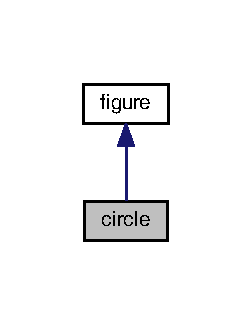
\includegraphics[width=121pt]{classcircle__inherit__graph}
\end{center}
\end{figure}


Collaboration diagram for circle\+:
\nopagebreak
\begin{figure}[H]
\begin{center}
\leavevmode
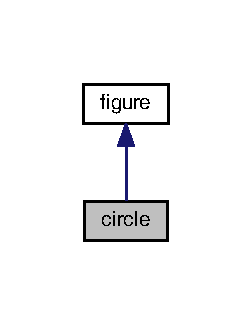
\includegraphics[width=121pt]{classcircle__coll__graph}
\end{center}
\end{figure}
\subsection*{Public Member Functions}
\begin{DoxyCompactItemize}
\item 
void \hyperlink{classcircle_aec30ad95a694a9f0f2cd149f38ae37ed}{show\+\_\+area} ()
\end{DoxyCompactItemize}
\subsection*{Additional Inherited Members}


\subsection{Member Function Documentation}
\index{circle@{circle}!show\+\_\+area@{show\+\_\+area}}
\index{show\+\_\+area@{show\+\_\+area}!circle@{circle}}
\subsubsection[{\texorpdfstring{show\+\_\+area()}{show_area()}}]{\setlength{\rightskip}{0pt plus 5cm}void circle\+::show\+\_\+area (
\begin{DoxyParamCaption}
{}
\end{DoxyParamCaption}
)\hspace{0.3cm}{\ttfamily [inline]}, {\ttfamily [virtual]}}\hypertarget{classcircle_aec30ad95a694a9f0f2cd149f38ae37ed}{}\label{classcircle_aec30ad95a694a9f0f2cd149f38ae37ed}


Reimplemented from \hyperlink{classfigure_acf1c18c0d61eeb3698d1e6883b910321}{figure}.


\begin{DoxyCode}
39                      \{
40       cout << \textcolor{stringliteral}{"Circle with radius "};
41       cout << \hyperlink{classfigure_adeb281a08de5069df09efe4e8b679557}{x};
42       cout << \textcolor{stringliteral}{" has an area of "};
43       cout << 3.14 * x * x << \textcolor{stringliteral}{".\(\backslash\)n"};
44     \}
\end{DoxyCode}


The documentation for this class was generated from the following file\+:\begin{DoxyCompactItemize}
\item 
\hyperlink{VirtualPoly_8cpp}{Virtual\+Poly.\+cpp}\end{DoxyCompactItemize}

\hypertarget{classfigure}{}\section{figure Class Reference}
\label{classfigure}\index{figure@{figure}}


Inheritance diagram for figure\+:
\nopagebreak
\begin{figure}[H]
\begin{center}
\leavevmode
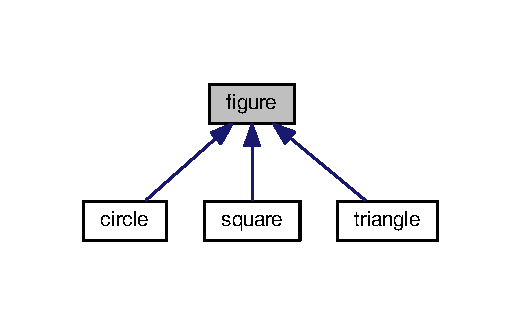
\includegraphics[width=250pt]{classfigure__inherit__graph}
\end{center}
\end{figure}
\subsection*{Public Member Functions}
\begin{DoxyCompactItemize}
\item 
void \hyperlink{classfigure_a422a3eae33671199a99e0a64bca92870}{set\+\_\+dim} (double i, double j=0)
\item 
virtual void \hyperlink{classfigure_acf1c18c0d61eeb3698d1e6883b910321}{show\+\_\+area} ()
\end{DoxyCompactItemize}
\subsection*{Protected Attributes}
\begin{DoxyCompactItemize}
\item 
double \hyperlink{classfigure_adeb281a08de5069df09efe4e8b679557}{x}
\item 
double \hyperlink{classfigure_aeb15782099be3fcb611f38ddd974fb37}{y}
\end{DoxyCompactItemize}


\subsection{Member Function Documentation}
\index{figure@{figure}!set\+\_\+dim@{set\+\_\+dim}}
\index{set\+\_\+dim@{set\+\_\+dim}!figure@{figure}}
\subsubsection[{\texorpdfstring{set\+\_\+dim(double i, double j=0)}{set_dim(double i, double j=0)}}]{\setlength{\rightskip}{0pt plus 5cm}void figure\+::set\+\_\+dim (
\begin{DoxyParamCaption}
\item[{double}]{i, }
\item[{double}]{j = {\ttfamily 0}}
\end{DoxyParamCaption}
)\hspace{0.3cm}{\ttfamily [inline]}}\hypertarget{classfigure_a422a3eae33671199a99e0a64bca92870}{}\label{classfigure_a422a3eae33671199a99e0a64bca92870}

\begin{DoxyCode}
8                                      \{
9     \hyperlink{classfigure_adeb281a08de5069df09efe4e8b679557}{x} = i;
10     \hyperlink{classfigure_aeb15782099be3fcb611f38ddd974fb37}{y} = j;
11   \}
\end{DoxyCode}
\index{figure@{figure}!show\+\_\+area@{show\+\_\+area}}
\index{show\+\_\+area@{show\+\_\+area}!figure@{figure}}
\subsubsection[{\texorpdfstring{show\+\_\+area()}{show_area()}}]{\setlength{\rightskip}{0pt plus 5cm}virtual void figure\+::show\+\_\+area (
\begin{DoxyParamCaption}
{}
\end{DoxyParamCaption}
)\hspace{0.3cm}{\ttfamily [inline]}, {\ttfamily [virtual]}}\hypertarget{classfigure_acf1c18c0d61eeb3698d1e6883b910321}{}\label{classfigure_acf1c18c0d61eeb3698d1e6883b910321}


Reimplemented in \hyperlink{classcircle_aec30ad95a694a9f0f2cd149f38ae37ed}{circle}, \hyperlink{classsquare_a11ed588dc4a0d7e47f11f077f57d1a16}{square}, and \hyperlink{classtriangle_af73356d9e4f6099ca599051e886378ae}{triangle}.


\begin{DoxyCode}
12                            \{
13     cout << \textcolor{stringliteral}{"No area computation defined "};
14     cout << \textcolor{stringliteral}{"for this class.\(\backslash\)n"};
15   \}
\end{DoxyCode}


\subsection{Member Data Documentation}
\index{figure@{figure}!x@{x}}
\index{x@{x}!figure@{figure}}
\subsubsection[{\texorpdfstring{x}{x}}]{\setlength{\rightskip}{0pt plus 5cm}double figure\+::x\hspace{0.3cm}{\ttfamily [protected]}}\hypertarget{classfigure_adeb281a08de5069df09efe4e8b679557}{}\label{classfigure_adeb281a08de5069df09efe4e8b679557}
\index{figure@{figure}!y@{y}}
\index{y@{y}!figure@{figure}}
\subsubsection[{\texorpdfstring{y}{y}}]{\setlength{\rightskip}{0pt plus 5cm}double figure\+::y\hspace{0.3cm}{\ttfamily [protected]}}\hypertarget{classfigure_aeb15782099be3fcb611f38ddd974fb37}{}\label{classfigure_aeb15782099be3fcb611f38ddd974fb37}


The documentation for this class was generated from the following file\+:\begin{DoxyCompactItemize}
\item 
\hyperlink{VirtualPoly_8cpp}{Virtual\+Poly.\+cpp}\end{DoxyCompactItemize}

\hypertarget{classsquare}{}\section{square Class Reference}
\label{classsquare}\index{square@{square}}


Inheritance diagram for square\+:
\nopagebreak
\begin{figure}[H]
\begin{center}
\leavevmode
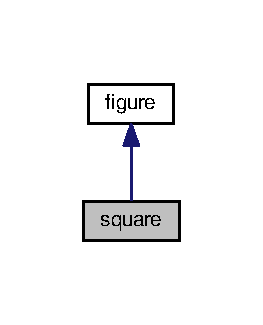
\includegraphics[width=126pt]{classsquare__inherit__graph}
\end{center}
\end{figure}


Collaboration diagram for square\+:
\nopagebreak
\begin{figure}[H]
\begin{center}
\leavevmode
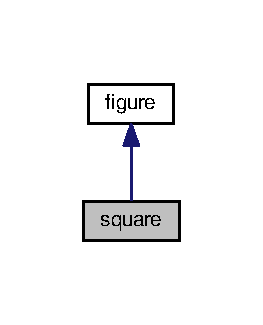
\includegraphics[width=126pt]{classsquare__coll__graph}
\end{center}
\end{figure}
\subsection*{Public Member Functions}
\begin{DoxyCompactItemize}
\item 
void \hyperlink{classsquare_a11ed588dc4a0d7e47f11f077f57d1a16}{show\+\_\+area} ()
\end{DoxyCompactItemize}
\subsection*{Additional Inherited Members}


\subsection{Member Function Documentation}
\index{square@{square}!show\+\_\+area@{show\+\_\+area}}
\index{show\+\_\+area@{show\+\_\+area}!square@{square}}
\subsubsection[{\texorpdfstring{show\+\_\+area()}{show_area()}}]{\setlength{\rightskip}{0pt plus 5cm}void square\+::show\+\_\+area (
\begin{DoxyParamCaption}
{}
\end{DoxyParamCaption}
)\hspace{0.3cm}{\ttfamily [inline]}, {\ttfamily [virtual]}}\hypertarget{classsquare_a11ed588dc4a0d7e47f11f077f57d1a16}{}\label{classsquare_a11ed588dc4a0d7e47f11f077f57d1a16}


Reimplemented from \hyperlink{classfigure_acf1c18c0d61eeb3698d1e6883b910321}{figure}.


\begin{DoxyCode}
30                      \{
31       cout << \textcolor{stringliteral}{"Square with dimensions "};
32       cout << \hyperlink{classfigure_adeb281a08de5069df09efe4e8b679557}{x} << \textcolor{stringliteral}{"x"} << \hyperlink{classfigure_aeb15782099be3fcb611f38ddd974fb37}{y};
33       cout << \textcolor{stringliteral}{" has an area of "};
34       cout << \hyperlink{classfigure_adeb281a08de5069df09efe4e8b679557}{x} *  y << \textcolor{stringliteral}{".\(\backslash\)n"};
35     \}
\end{DoxyCode}


The documentation for this class was generated from the following file\+:\begin{DoxyCompactItemize}
\item 
\hyperlink{VirtualPoly_8cpp}{Virtual\+Poly.\+cpp}\end{DoxyCompactItemize}

\hypertarget{classtriangle}{}\section{triangle Class Reference}
\label{classtriangle}\index{triangle@{triangle}}


Inheritance diagram for triangle\+:
\nopagebreak
\begin{figure}[H]
\begin{center}
\leavevmode
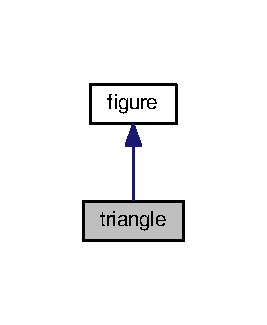
\includegraphics[width=128pt]{classtriangle__inherit__graph}
\end{center}
\end{figure}


Collaboration diagram for triangle\+:
\nopagebreak
\begin{figure}[H]
\begin{center}
\leavevmode
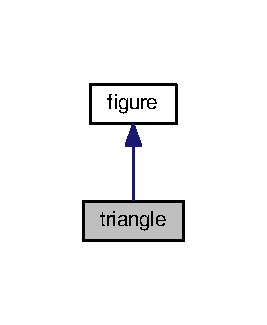
\includegraphics[width=128pt]{classtriangle__coll__graph}
\end{center}
\end{figure}
\subsection*{Public Member Functions}
\begin{DoxyCompactItemize}
\item 
void \hyperlink{classtriangle_af73356d9e4f6099ca599051e886378ae}{show\+\_\+area} ()
\end{DoxyCompactItemize}
\subsection*{Additional Inherited Members}


\subsection{Member Function Documentation}
\index{triangle@{triangle}!show\+\_\+area@{show\+\_\+area}}
\index{show\+\_\+area@{show\+\_\+area}!triangle@{triangle}}
\subsubsection[{\texorpdfstring{show\+\_\+area()}{show_area()}}]{\setlength{\rightskip}{0pt plus 5cm}void triangle\+::show\+\_\+area (
\begin{DoxyParamCaption}
{}
\end{DoxyParamCaption}
)\hspace{0.3cm}{\ttfamily [inline]}, {\ttfamily [virtual]}}\hypertarget{classtriangle_af73356d9e4f6099ca599051e886378ae}{}\label{classtriangle_af73356d9e4f6099ca599051e886378ae}


Reimplemented from \hyperlink{classfigure_acf1c18c0d61eeb3698d1e6883b910321}{figure}.


\begin{DoxyCode}
20                      \{
21       cout << \textcolor{stringliteral}{"Triangle with height "};
22       cout << \hyperlink{classfigure_adeb281a08de5069df09efe4e8b679557}{x} << \textcolor{stringliteral}{" and base "} << \hyperlink{classfigure_aeb15782099be3fcb611f38ddd974fb37}{y};
23       cout << \textcolor{stringliteral}{" has an area of "};
24       cout << \hyperlink{classfigure_adeb281a08de5069df09efe4e8b679557}{x} * 0.5 * y << \textcolor{stringliteral}{".\(\backslash\)n"};
25     \}
\end{DoxyCode}


The documentation for this class was generated from the following file\+:\begin{DoxyCompactItemize}
\item 
\hyperlink{VirtualPoly_8cpp}{Virtual\+Poly.\+cpp}\end{DoxyCompactItemize}

\chapter{File Documentation}
\hypertarget{VirtualPoly_8cpp}{}\section{Virtual\+Poly.\+cpp File Reference}
\label{VirtualPoly_8cpp}\index{Virtual\+Poly.\+cpp@{Virtual\+Poly.\+cpp}}
{\ttfamily \#include $<$iostream$>$}\\*
Include dependency graph for Virtual\+Poly.\+cpp\+:
\nopagebreak
\begin{figure}[H]
\begin{center}
\leavevmode
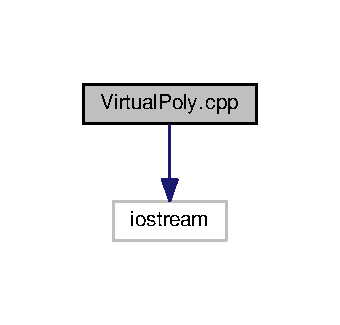
\includegraphics[width=163pt]{VirtualPoly_8cpp__incl}
\end{center}
\end{figure}
\subsection*{Classes}
\begin{DoxyCompactItemize}
\item 
class \hyperlink{classfigure}{figure}
\item 
class \hyperlink{classtriangle}{triangle}
\item 
class \hyperlink{classsquare}{square}
\item 
class \hyperlink{classcircle}{circle}
\end{DoxyCompactItemize}
\subsection*{Functions}
\begin{DoxyCompactItemize}
\item 
int \hyperlink{VirtualPoly_8cpp_ae66f6b31b5ad750f1fe042a706a4e3d4}{main} ()
\end{DoxyCompactItemize}


\subsection{Function Documentation}
\index{Virtual\+Poly.\+cpp@{Virtual\+Poly.\+cpp}!main@{main}}
\index{main@{main}!Virtual\+Poly.\+cpp@{Virtual\+Poly.\+cpp}}
\subsubsection[{\texorpdfstring{main()}{main()}}]{\setlength{\rightskip}{0pt plus 5cm}int main (
\begin{DoxyParamCaption}
{}
\end{DoxyParamCaption}
)}\hypertarget{VirtualPoly_8cpp_ae66f6b31b5ad750f1fe042a706a4e3d4}{}\label{VirtualPoly_8cpp_ae66f6b31b5ad750f1fe042a706a4e3d4}

\begin{DoxyCode}
48 \{
49   \hyperlink{classfigure}{figure} *p; \textcolor{comment}{// create a pointer to base type}
50 
51   \hyperlink{classtriangle}{triangle} t; \textcolor{comment}{// create objects of derived types}
52   \hyperlink{classsquare}{square} s;
53   \hyperlink{classcircle}{circle} c;
54 
55   p = &t;
56   p->\hyperlink{classfigure_a422a3eae33671199a99e0a64bca92870}{set\_dim}(10.0, 5.0);
57   p->\hyperlink{classfigure_acf1c18c0d61eeb3698d1e6883b910321}{show\_area}();
58 
59   p = &s;
60   p->\hyperlink{classfigure_a422a3eae33671199a99e0a64bca92870}{set\_dim}(10.0, 5.0);
61   p->\hyperlink{classfigure_acf1c18c0d61eeb3698d1e6883b910321}{show\_area}();
62 
63   p = &c;
64   p->\hyperlink{classfigure_a422a3eae33671199a99e0a64bca92870}{set\_dim}(9.0);
65   p->\hyperlink{classfigure_acf1c18c0d61eeb3698d1e6883b910321}{show\_area}();
66 
67   \textcolor{keywordflow}{return} 0;
68 \}\end{DoxyCode}


Here is the call graph for this function\+:
\nopagebreak
\begin{figure}[H]
\begin{center}
\leavevmode
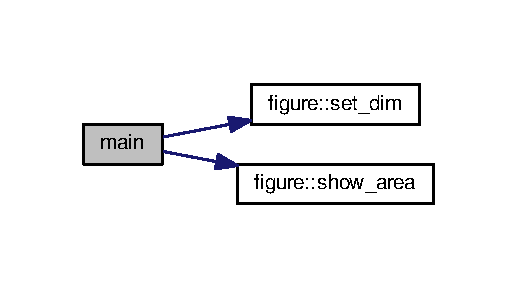
\includegraphics[width=248pt]{VirtualPoly_8cpp_ae66f6b31b5ad750f1fe042a706a4e3d4_cgraph}
\end{center}
\end{figure}



%--- End generated contents ---

% Index
\backmatter
\newpage
\phantomsection
\clearemptydoublepage
\addcontentsline{toc}{chapter}{Index}
\printindex

\end{document}
